% answers.tex —— 2008 年·全国大纲卷Ⅱ·理科 · 参考答案与详细解析片段
% 由 tools/generate_projects.py 依来源总账自 2008/2008_数学真题_全国2理_试题.md + 2008/2008_数学真题_全国2理_解析正文.md + 2008/2008_数学真题_全国2理_答案要点.md 生成，勿手改（改源 MD 后重跑）


\begin{gktip}
固定源 PDF 为印刷页码 437–438 的两页题面，不附答案。以下解析均依据固定源独立复算；第 19 题图形在 LaTeX 工程中以 TikZ/PGFPlots 矢量源重绘。
\end{gktip}

\begin{answer}
\gksolhead{1}{}

\textbf{题目}：

设集合 $M=\{m\in\mathbb Z\mid-3<m<2\}$，$N=\{n\in\mathbb Z\mid-1\leqslant n\leqslant3\}$，则 $M\cap N=$\mbox{（　　）}

（A）$\{0,1\}$\quad（B）$\{-1,0,1\}$\quad（C）$\{0,1,2\}$\quad（D）$\{-1,0,1,2\}$

\Needspace{4\baselineskip}
\textbf{解析}

$M=\{-2,-1,0,1\}$，$N=\{-1,0,1,2,3\}$，故交集为 $\{-1,0,1\}$，选 B。

\gkanswer{答案：B}

\end{answer}
\begin{answer}
\gksolhead{2}{}

\textbf{题目}：

设 $a,b\in\mathbb R$ 且 $b\ne0$，若复数 $(a+b\mathrm i)^3$ 是实数，则\mbox{（　　）}

（A）$b^2=3a^2$\quad（B）$a^2=3b^2$\quad（C）$b^2=9a^2$\quad（D）$a^2=9b^2$

\Needspace{4\baselineskip}
\textbf{解析}

令 $z=a+b\mathrm i$。$z^3$ 为实数且 $b\ne0$，故 $z$ 的辐角为 $\pi/3$ 或 $2\pi/3$（模 $\pi/3$），从而 $\lvert b/a\rvert=\sqrt3$，即 $a^2=3b^2$，选 B。

\gkanswer{答案：C}

\end{answer}
\begin{answer}
\gksolhead{3}{}

\textbf{题目}：

函数 $f(x)=\dfrac1x-x$ 的图象关于\mbox{（　　）}

（A）$y$ 轴对称\quad（B）直线 $y=-x$ 对称\quad（C）坐标原点对称\quad（D）直线 $y=x$ 对称

\Needspace{4\baselineskip}
\textbf{解析}

$f(-x)=-f(x)$，图象关于原点对称，选 C。

\gkanswer{答案：C}

\end{answer}
\begin{answer}
\gksolhead{4}{}

\textbf{题目}：

若 $x\in(e^{-1},1)$，$a=\ln x$，$b=2\ln x$，$c=\ln^3x$，则\mbox{（　　）}

（A）$a<b<c$\quad（B）$c<a<b$\quad（C）$b<a<c$\quad（D）$b<c<a$

\Needspace{4\baselineskip}
\textbf{解析}

令 $t=\ln x\in(-1,0)$，则 $a=t,b=2t,c=t^3$，比较得 $b<c<a$，选 D。

\gkanswer{答案：D}

\end{answer}
\begin{answer}
\gksolhead{5}{}

\textbf{题目}：

\Needspace{5\baselineskip}
设变量 $x,y$ 满足约束条件

\nopagebreak[4]
\[
\begin{cases}
y\geqslant x,\\
x+2y\leqslant2,\\
x\geqslant-2,
\end{cases}
\]

则 $z=x-3y$ 的最小值为\mbox{（　　）}

（A）$-2$\quad（B）$-4$\quad（C）$-6$\quad（D）$-8$

\Needspace{4\baselineskip}
\textbf{解析}

在上边界 $y=1-x/2$ 上，$z=x-3y=5x/2-3$，在 $x\geqslant-2$ 上最小值为 $-8$，选 D。

\gkanswer{答案：D}

\end{answer}
\begin{answer}
\gksolhead{6}{}

\textbf{题目}：

从 $20$ 名男同学、$10$ 名女同学中任选 $3$ 名参加体能测试，则选到的 $3$ 名同学中既有男同学又有女同学的概率为\mbox{（　　）}

（A）$\dfrac9{29}$\quad（B）$\dfrac{10}{29}$\quad（C）$\dfrac{19}{29}$\quad（D）$\dfrac{20}{29}$

\Needspace{4\baselineskip}
\textbf{解析}

\Needspace{5\baselineskip}
总选法 $\binom{30}{3}$，减去全男与全女：

\nopagebreak[4]
\[
1-\frac{\binom{20}{3}+\binom{10}{3}}{\binom{30}{3}}
=\frac{19}{29}
\]

选 C。

\gkanswer{答案：C}

\end{answer}
\begin{answer}
\gksolhead{7}{}

\textbf{题目}：

$(1-\sqrt{x})^6(1+\sqrt{x})^4$ 的展开式中 $x$ 的系数是\mbox{（　　）}

（A）$-4$\quad（B）$-3$\quad（C）$3$\quad（D）$4$

\Needspace{4\baselineskip}
\textbf{解析}

$(1-\sqrt x)^6(1+\sqrt x)^4=(1-\sqrt x)^2(1-x)^4$，取 $x$ 项得系数 $-4$，选 A。

\gkanswer{答案：A}

\end{answer}
\begin{answer}
\gksolhead{8}{}

\textbf{题目}：

若动直线 $x=a$ 与函数 $f(x)=\sin x$ 和 $g(x)=\cos x$ 的图象分别交于 $M\text{、}N$ 两点，则 $|MN|$ 的最大值为\mbox{（　　）}

（A）$1$\quad（B）$\sqrt2$\quad（C）$\sqrt3$\quad（D）$2$

\Needspace{4\baselineskip}
\textbf{解析}

\Needspace{5\baselineskip}
两交点纵坐标为 $\sin a,\cos a$，故

\nopagebreak[4]
\[
|MN|=|\sin a-\cos a|\leqslant\sqrt2
\]

选 B。

\gkanswer{答案：B}

\end{answer}
\begin{answer}
\gksolhead{9}{}

\textbf{题目}：

设 $a>1$，则双曲线 $\dfrac{x^2}{a^2}-\dfrac{y^2}{(a+1)^2}=1$ 的离心率 $e$ 的取值范围是\mbox{（　　）}

（A）$(\sqrt2,2)$\quad（B）$(\sqrt2,\sqrt5)$\quad（C）$(2,\sqrt5)$\quad（D）$(2,\sqrt5]$

\Needspace{4\baselineskip}
\textbf{解析}

\Needspace{5\baselineskip}
双曲线离心率满足

\nopagebreak[4]
\[
e^2=1+\frac{(a+1)^2}{a^2}
=2+\frac2a+\frac1{a^2}
\]

$a>1$，故 $\sqrt2<e<\sqrt5$，选 B。

\gkanswer{答案：B}

\end{answer}
\begin{answer}
\gksolhead{10}{}

\textbf{题目}：

已知正四棱锥 $S-ABCD$ 的侧棱长与底面边长相等，$E$ 是 $SB$ 的中点，则 $AE\text{、}SD$ 所成的角的余弦值为\mbox{（　　）}

（A）$\dfrac13$\quad（B）$\dfrac{\sqrt2}{3}$\quad（C）$\dfrac{\sqrt3}{3}$\quad（D）$\dfrac23$

\Needspace{4\baselineskip}
\textbf{解析}

取正四棱锥底面边长和侧棱长均为 $1$，设底面中心为原点，直接计算 $\overrightarrow{AE}$ 与 $\overrightarrow{SD}$ 的内积及长度，得余弦为 $1/3$，选 A。

\gkanswer{答案：A}

\end{answer}
\begin{answer}
\gksolhead{11}{}

\textbf{题目}：

等腰三角形两腰所在直线的方程分别为 $x+y-2=0$ 与 $x-7y-4=0$，原点在等腰三角形的底边上，则底边所在直线的斜率为\mbox{（　　）}

（A）$3$\quad（B）$2$\quad（C）$-\dfrac13$\quad（D）$-\dfrac12$

\Needspace{4\baselineskip}
\textbf{解析}

两腰直线交于顶点，原点在底边上。由等腰条件和两条腰的对称关系求得底边斜率为 $-1/3$，选 C。

\gkanswer{答案：C}

\end{answer}
\begin{answer}
\gksolhead{12}{}

\textbf{题目}：

已知球的半径为 $2$，相互垂直的两个平面分别截球面得两个圆。若两圆的公共弦长为 $2$，则两圆的圆心距等于\mbox{（　　）}

（A）$1$\quad（B）$\sqrt2$\quad（C）$\sqrt3$\quad（D）$2$

\Needspace{4\baselineskip}
\textbf{解析}

与全国Ⅱ文科第 12 题相同，两圆圆心距平方为 $d_1^2+d_2^2=3$，故圆心距为 $\sqrt3$，选 C。

\gkanswer{答案：C}

\end{answer}
\begin{answer}
\gksolhead{13}{}

\textbf{题目}：

设向量 $\boldsymbol a=(1,2)$，$\boldsymbol b=(2,3)$。若向量 $\lambda\boldsymbol a+\boldsymbol b$ 与向量 $\boldsymbol c=(-4,-7)$ 共线，则 $\lambda=$\gkblank{}。

\Needspace{4\baselineskip}
\textbf{解析}

\Needspace{5\baselineskip}
共线行列式给出

\nopagebreak[4]
\[
\begin{vmatrix}\lambda+2&2\lambda+3\\-4&-7\end{vmatrix}=0
\]

解得 $\lambda=2$。

\gkanswer{答案：$2$}

\end{answer}
\begin{answer}
\gksolhead{14}{}

\textbf{题目}：

设曲线 $y=e^{ax}$ 在点 $(0,1)$ 处的切线与直线 $x+2y+1=0$ 垂直，则 $a=$\gkblank{}。

\Needspace{4\baselineskip}
\textbf{解析}

$y=e^{ax}$ 在 $(0,1)$ 处切线斜率为 $a$。直线 $x+2y+1=0$ 斜率为 $-1/2$，垂直条件给出 $a=2$。

\gkanswer{答案：$2$}

\end{answer}
\begin{answer}
\gksolhead{15}{}

\textbf{题目}：

已知 $F$ 是抛物线 $C:y^2=4x$ 的焦点，过 $F$ 且斜率为 $1$ 的直线交 $C$ 于 $A\text{、}B$ 两点。设 $|FA|>|FB|$，则 $|FA|$ 与 $|FB|$ 的比值等于\gkblank{}。

\Needspace{4\baselineskip}
\textbf{解析}

\Needspace{5\baselineskip}
焦点为 $(1,0)$，过焦点且斜率为 $1$ 的直线为 $y=x-1$。与 $y^2=4x$ 联立得 $x=3\pm2\sqrt2$。抛物线上的点到焦点距离为 $x+1$，故比值为

\nopagebreak[4]
\[
\frac{4+2\sqrt2}{4-2\sqrt2}=3+2\sqrt2
\]

\gkanswer{答案：$3+2\sqrt2$。}

\end{answer}
\begin{answer}
\gksolhead{16}{}

\textbf{题目}：

平面内的一个四边形为平行四边形的充要条件有多个，如两组对边分别平行。类似地，写出空间中的一个四棱柱为平行六面体的两个充要条件：充要条件①\gkblank{}；充要条件②\gkblank{}。（写出你认为正确的两个充要条件）

\Needspace{4\baselineskip}
\textbf{解析}

可取两个充要条件：两个底面都是平行四边形；任意两个相邻侧面都是平行四边形。

\gkanswer{答案：两组相对的侧面分别为平行四边形；两个底面都是平行四边形。}

\end{answer}
\begin{answer}
\gksolhead{17}{}

\textbf{题目}：

在 $\triangle ABC$ 中，$\cos B=-\dfrac5{13}$，$\cos C=\dfrac45$。

（1） 求 $\sin A$ 的值；

（2） 设 $\triangle ABC$ 的面积 $S_{\triangle ABC}=\dfrac{33}{2}$，求 $BC$ 的长。

\Needspace{4\baselineskip}
\textbf{解析}

\gksubpart{(1)}

\Needspace{5\baselineskip}
$\sin B=12/13$，$\sin C=3/5$，故

\nopagebreak[4]
\[
\sin A=\sin(B+C)=\sin B\cos C+\cos B\sin C
=\frac{12}{13}\cdot\frac45-\frac5{13}\cdot\frac35
=\frac{33}{65}
\]

\gksubpart{(2)}

\Needspace{5\baselineskip}
由正弦定理 $a:b:c=11:20:13$。设比例因子为 $k$，则

\nopagebreak[4]
\[
S=\frac12ab\sin C
=\frac12(11k)(20k)\frac35
=66k^2=\frac{33}{2}
\]

故 $k=1/2$，$BC=a=11/2$。

\gkanswer{答案（1）：$\sin A=\dfrac{33}{65}$。}

\gkanswer{答案（2）：$BC=\dfrac{11}{2}$。}

\end{answer}
\begin{answer}
\gksolhead{18}{}

\textbf{题目}：

购买某种保险，每个投保人每年度向保险公司交纳保费 $a$ 元，若投保人在购买保险的一年度内出险，则可以获得 $10000$ 元的赔偿金。假定在一年度内有 $10000$ 人购买了这种保险，且各投保人是否出险相互独立。已知保险公司在一年度内至少支付赔偿金 $10000$ 元的概率为 $1-0.999^{10000}$。

（1） 求一投保人在一年度内出险的概率 $p$；

（2） 设保险公司开办该项险种业务除赔偿金外的成本为 $50000$ 元，为保证盈利的期望不小于 $0$，求每位投保人应交纳的最低保费。（单位：元）

\Needspace{4\baselineskip}
\textbf{解析}

\gksubpart{(1)}

至少支付一次赔偿的概率为 $1-(1-p)^{10000}$，与题设比较得 $1-p=0.999$，故 $p=0.001$。

\gksubpart{(2)}

\Needspace{5\baselineskip}
每位投保人的期望赔偿为 $10000p=10$ 元，万人总期望赔偿为 $100000$ 元，加上成本 $50000$ 元，故

\nopagebreak[4]
\[
10000a-100000-50000\geqslant0
\]

所以 $a\geqslant15$。

\gkanswer{答案（1）：$p=0.001$。}

\gkanswer{答案（2）：每位投保人的最低保费为 $15$ 元。}

\end{answer}
\begin{answer}
\gksolhead{19}{}

\textbf{题目}：

如图，正四棱柱 $ABCD-A_1B_1C_1D_1$ 中，$AA_1=2AB=4$，点 $E$ 在 $CC_1$ 上且 $C_1E=3EC$。
\nopagebreak[4]
\begin{center}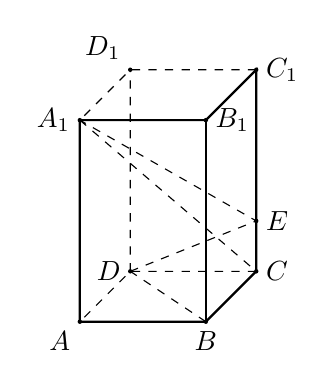
\begin{tikzpicture}[scale=.8,>=stealth]
\coordinate (A) at (0,0); \coordinate (B) at (2,0);
\coordinate (C) at (2.8,.8); \coordinate (D) at (.8,.8);
\coordinate (A1) at (0,3.2); \coordinate (B1) at (2,3.2);
\coordinate (C1) at (2.8,4); \coordinate (D1) at (.8,4);
\coordinate (E) at (2.8,1.6);
\draw[thick] (A)--(B)--(C)--(C1)--(B1)--(A1)--cycle;
\draw[dashed] (C)--(D)--(A) (C1)--(D1)--(A1) (D)--(D1);
\draw[thick] (B)--(B1) (C)--(C1);
\draw[dashed] (A1)--(C) (B)--(D) (D)--(E)--(A1);
\fill (A) circle (1pt) node[below left] {$A$};
\fill (B) circle (1pt) node[below] {$B$};
\fill (C) circle (1pt) node[right] {$C$};
\fill (D) circle (1pt) node[left] {$D$};
\fill (A1) circle (1pt) node[left] {$A_1$};
\fill (B1) circle (1pt) node[right] {$B_1$};
\fill (C1) circle (1pt) node[right] {$C_1$};
\fill (D1) circle (1pt) node[above left] {$D_1$};
\fill (E) circle (1pt) node[right] {$E$};
\end{tikzpicture}
\end{center}
\nopagebreak[4]
（1） 证明：$A_1C\perp$ 平面 $BED$；

（2） 求二面角 $A_1-DE-B$ 的大小。

\Needspace{4\baselineskip}
\textbf{解析}

\gksubpart{(1)}

取 $A=(0,0,0),B=(2,0,0),C=(2,2,0),D=(0,2,0)$，$A_1=(0,0,4)$，由 $C_1E=3EC$ 得 $E=(2,2,1)$。计算 $\overrightarrow{A_1C}$ 与 $\overrightarrow{BE},\overrightarrow{BD}$ 的内积均为零，故 $A_1C\perp$ 平面 $BED$。

\gksubpart{(2)}

\Needspace{5\baselineskip}
取平面 $A_1DE$、$BDE$ 的法向量，内积计算得

\nopagebreak[4]
\[
\cos\theta=\frac1{\sqrt{126}}
\]

\gkanswer{答案（1）：见解析版}

\gkanswer{答案（2）：二面角 $A_1-DE-B$ 的余弦为 $\dfrac1{\sqrt{126}}$。}

\end{answer}
\begin{answer}
\gksolhead{20}{}

\textbf{题目}：

设数列 $\{a_n\}$ 的前 $n$ 项和为 $S_n$。已知 $a_1=a$，$a_{n+1}=S_n+3^n$，$n\in\mathbb N^*$。

（1） 设 $b_n=S_n-3^n$，求数列 $\{b_n\}$ 的通项公式；

（2） 若 $a_{n+1}\geqslant a_n$，$n\in\mathbb N^*$，求 $a$ 的取值范围。

\Needspace{4\baselineskip}
\textbf{解析}

\gksubpart{(1)}

\Needspace{5\baselineskip}
由 $b_n=S_n-3^n$ 及 $a_{n+1}=S_n+3^n$，有

\nopagebreak[4]
\[
b_{n+1}=S_{n+1}-3^{n+1}=2(S_n-3^n)=2b_n
\]

且 $b_1=a-3$，故 $b_n=(a-3)2^{n-1}$。

\gksubpart{(2)}

\Needspace{5\baselineskip}
对 $n\geqslant2$，由 $a_n=S_n-S_{n-1}$ 得

\nopagebreak[4]
\[
a_n=(a-3)2^{n-2}+2\cdot3^{n-1}
\]

于是 $a_{n+1}-a_n\geqslant0$ 的最严格条件出现在 $n=2$，给出 $a+9\geqslant0$，故 $a\geqslant-9$。

\gkanswer{答案（1）：$b_n=(a-3)2^{n-1}$。}

\gkanswer{答案（2）：$a\geqslant-9$。}

\end{answer}
\begin{answer}
\gksolhead{21}{}

\textbf{题目}：

设椭圆中心在坐标原点，$A(2,0)$、$B(0,1)$ 是它的两个顶点，直线 $y=kx$（$k>0$）与 $AB$ 相交于点 $D$，与椭圆相交于 $E\text{、}F$ 两点。

（1） 若 $\overline{ED}=6\overline{DF}$，求 $k$ 的值；

（2） 求四边形 $AEBF$ 面积的最大值。

\Needspace{4\baselineskip}
\textbf{解析}

\gksubpart{(1)}

\Needspace{5\baselineskip}
直线 $y=kx$ 与椭圆交点的横坐标为 $\pm r$，其中 $r=2/\sqrt{1+4k^2}$。将 $D$ 坐标代入向量比例 $\overrightarrow{ED}=6\overrightarrow{DF}$，得

\nopagebreak[4]
\[
24k^2-25k+6=0
\]

故 $k=2/3$ 或 $k=3/8$。

\gksubpart{(2)}

\Needspace{5\baselineskip}
四边形面积化为

\nopagebreak[4]
\[
S(k)=\frac{2(2k+1)}{\sqrt{1+4k^2}}
\]

在 $k=1/2$ 处取最大值 $2\sqrt2$。

\gkanswer{答案（1）：$k=\dfrac23$ 或 $k=\dfrac38$。}

\gkanswer{答案（2）：四边形 $AEBF$ 面积的最大值为 $2\sqrt2$。}

\end{answer}
\begin{answer}
\gksolhead{22}{}

\textbf{题目}：

设函数 $f(x)=\dfrac{\sin x}{2+\cos x}$。

（1） 求 $f(x)$ 的单调区间；

（2） 如果对任何 $x\geqslant0$，都有 $f(x)\leqslant ax$，求 $a$ 的取值范围。

\Needspace{4\baselineskip}
\textbf{解析}

\gksubpart{(1)}

\nopagebreak[4]
\[
f'(x)=\frac{2\cos x+1}{(2+\cos x)^2}
\]

所以 $f$ 在 $\cos x>-1/2$ 的区间递增，在 $\cos x<-1/2$ 的区间递减。

\gksubpart{(2)}

当 $x\to0^+$ 时 $f(x)/x\to1/3$，且可由 $2+\cos x\geqslant1$ 验证 $f(x)\leqslant x/3$ 对 $x\geqslant0$ 成立，故充要条件为 $a\geqslant1/3$。

\gkanswer{答案（1）：$f(x)$ 在 $\cos x>-\dfrac12$ 的区间上递增，在 $\cos x<-\dfrac12$ 的区间上递减。}

\gkanswer{答案（2）：$a\geqslant\dfrac13$。}

\end{answer}